\chapter{Wprowadzenie}
\label{cha:wprowadzenie}
\section{Historia robotów kroczących}
Pierwsza idea robota kroczącego pojawiła się już pod koniec XV wieku, a narodziła się w głowie nikogo innego jak Leonarda Da Vinci. Od tamtej pory wielu naukowców próbowało tworzyć konstrukcje, które używały nóg zamiast kół. Jednakże, pierwsze faktycznie udane roboty tego typu datuje się dopiero na początek lat 60 ubiegłego wieku. Pojawiły sie wtedy pierwsze działające konstrukcje, na przykład robot czteronożny zbudowany przez Josepha Shingleya oraz roboty sześcio i ośmonożne zbudowane przez "Space General Corporation". \cite{history}\\

Od tamtej pory powstało wiele różnych projektów, które kategoryzuje się w zależności od ilości nóg posiadanych przez robota:
\begin{itemize}[noitemsep]
\item jednonożne,
\item dwunożne (Humanoid, chicken-walkers),
\item czteronożne (Quadrupedal),
\item sześcionożne (Hexapod),
\item ośmionożne,
\item gąsiennicowe.
\end{itemize}

Można tu zaobserwować pewną tendencję spadkową, wraz z upływem czasu widać wzrost udanych konstrukcji o mniejszej liczbie nóg. Konstrukcje takie wymagają większej wiedzy naukowców, lepiej dobranych algorytmów ale za to można je skonstruować mniejszym nakładem materiałowym. Stąd naturalne jest dążenie do ograniczania liczby nóg w konstrukcjach robotów kroczących\\

Pojawia się także inna tendencja w ilości nóg robotów. Prawie wszystkie konstrukcje (poza jednonożnymi) opierają się na anatomii zwierząt. Jest to raczej logiczna tendencja, jako że do takich robotów mamy już algorytmy chodu opracowane przez miliony lat ewolucji. Biologiczne "konstrukcje", które nie mają sensu nie przetrwałyby do dziś. \cite{history}\\

Co natomiast z konstrucjami robotów trójnożnych? Można się zastanowić czy konstrukcje takie nie powstają ponieważ faktycznie nie mają sensu, czy może dlatego że temat bardziej "klasycznych", prostszych w implementacji, konstrukcji nie został po prostu jeszcze wyczerpany przez naukowców. Jeżeli rozejrzymy się dookoła siebie możemy zaobserwować wiele przedmiotów codziennego użytku które posiadają właśnie trzy nogi, od wszelakich taboretów, przez wieszaki na ubrania po stoły. Są to jednak przedmioty statyczne i dla takich rozwiązań trzy nogi są wymaganym minimum aby dany przedmiot stał stabilnie. Co jednak z konstrukcjami dynamicznymi? Jeżeli robot trójnożny podniesie nogę, straci stabilność, zacznie się przewracać. Czyni to z niego dość ciekawą konstrukcję, gdzie w momencie stania w miejscu zachowuje się bardzej jak roboty o większej ilości nóg, nie przewraca się, a podczas ruchu zachowuje się jak roboty dwunożne, musi odpowiednio szybko odstawić nogę w odpowiednie miejsce aby się nie przewrócić.\\

\section{Istniejące konstrukcje trójnożne}
Konstrukcje trójnożne pojawiały się w dziełach science fiction już od dawna, od "The War of the Worlds" z 1898 aż po "Mroczne Widmo" z 2001 i regularnie pojawiają się naukowcy, którzy próbują udowodnić że nie trzeba ogarniczać tego typu robotów do dzieł z obszaru science fiction.\\
\subsection{STriDER}
\begin{figure}[h!]
\centering
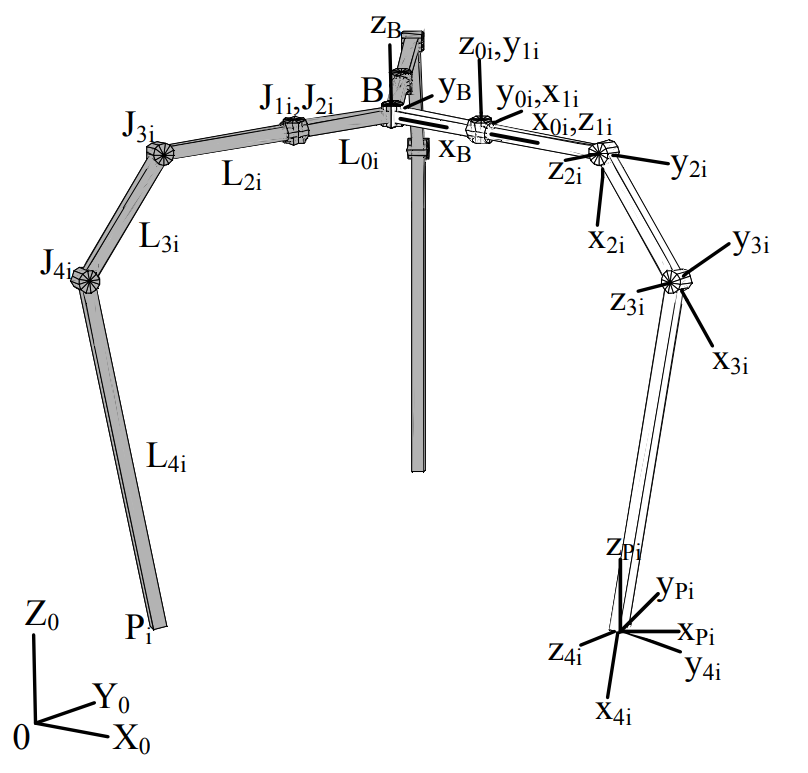
\includegraphics[width=0.5\textwidth]{img/strider_photo.png}
\caption{Schemat kinematyczny robota Strider źródło: \cite{strider}}
\label{martian_photo}
\end{figure}
Został zbudowany w 2007 na Uniwersytecie Stanowym w Virginii. Jego celem były eksperymenty z algorytmami chodu i doclewo, prowadzenie obserwacji. Miały to umożliwić długie nogi, które znacznie podwyższały konstrukcję i sprawiały że górna platforma była idealna do instalowania wszelakiego rodzaju urządzęń typu kamery. Kinematykę robota można określić jako $3-SRRR$, a kinematykę jednej nogi jako $RRR$. Przy czym "pierwsze" $R$ oznacza obrót dookoła osi $x$ a dwa kolejne $R$ oznaczają obrót wokół osi $y$ (zgodnie z oznaczeniami na rysunku \ref{strider_math})  \cite{strider}\\

\begin{figure}[h!]
\centering
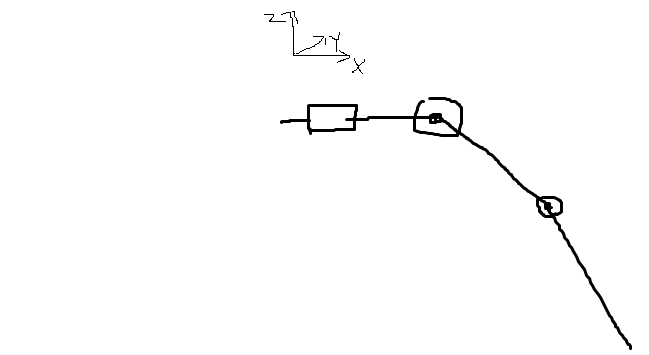
\includegraphics[width=\textwidth]{img/strider_math.png}
\caption{Uproszczony model matematyczny nogi robota STriDER}
\label{strider_math}
\end{figure}

\subsection{Triped Martian}
\begin{figure}[h!]
\centering
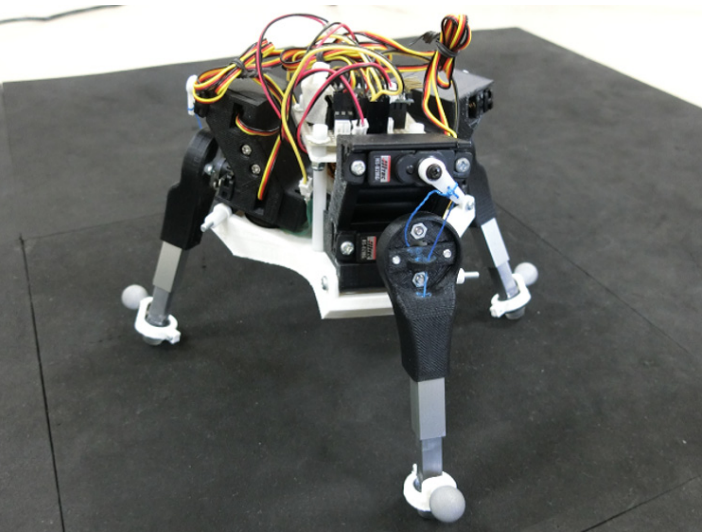
\includegraphics[width=0.5\textwidth]{img/martian_photo.png}
\caption{Zdjęcie robota Martian źródło: \cite{Triped_Martian}}
\label{martian_photo}
\end{figure}
Jest to robot zbudowany przez Yoichi Masudę na uniwersytecie w Osace w 2017 roku. Kinematyka tego robota opiera się na mechaniźmie SLIP (Spring-Loaded-Inverted Pendulum). SLIP ma w pewien sposób symulować sposób poruszania się stosowany przez ludzi i zwierzęta. Sprężyna wewnątrz nogi robota jest naciągana, co powoduje skracanie się nogi, a zwalnianie sprężyny z powrotem wydłuża człon. Dodatkowo dodane jest serwo, które może obracać nogę dookoła osi $y$. Czyni to z nogi robota mechanizm o kinematyce typu $RL$. Został także dodany czujnik naprężenia, który jest w stanie zmierzyć siłę naciągu nici kompresującej sprężynę. \cite{Triped_Martian}\\

\begin{figure}[h!]
\centering
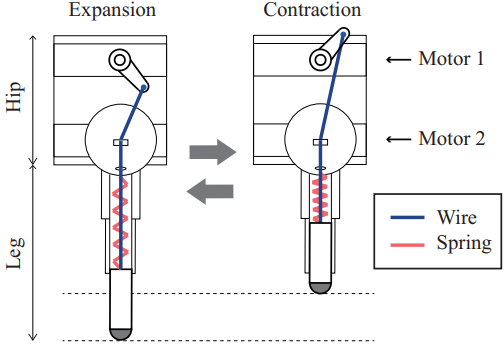
\includegraphics[width=0.5\textwidth]{img/martian_model.png}
\caption{Model nogi robota Triped Martian źródło: \cite{Triped_Martian}}
\label{martian_leg}
\end{figure}

\subsection{Inne konstrukcje}
W internecie można także znaleźć kilka różnych, niezbyt dobrze udokumentowanych konstrukcji zakończonych mniejszym lub większym sukcesem:
\begin{itemize}[noitemsep]
\item Makerfaire 3-legged walking robot \cite{makerfaire_three_legged}%\href{https://makerfaire.com/maker/entry/71669/}{Makerfaire 3-legged walking robot}
\item Missel tripod robot \cite{Missel_tripod}%\href{https://youtu.be/HGEhCCUgFMg}{missel tripod robot}
\end{itemize}

Niestety konstrukcje te nie posiadają żadnej dokumentacji technicznej i nie da się dokładnie określić zasady ich działania. Nie można nawet mieć pewności że konstrukcje te faktycznie istnieją a nie są oszustwem lub inną formą naginania rzeczywistości, na co mogłaby wskazywać jakość filmików i uboga ilość materiałów.\\